% TEMPLATE for Usenix papers, specifically to meet requirements of
%  USENIX '05
% originally a template for producing IEEE-format articles using LaTeX.
%   written by Matthew Ward, CS Department, Worcester Polytechnic Institute.
% adapted by David Beazley for his excellent SWIG paper in Proceedings,
%   Tcl 96
% turned into a smartass generic template by De Clarke, with thanks to
%   both the above pioneers
% use at your own risk.  Complaints to /dev/null.
% make it two column with no page numbering, default is 10 point

% Munged by Fred Douglis <douglis@research.att.com> 10/97 to separate
% the .sty file from the LaTeX source template, so that people can
% more easily include the .sty file into an existing document.  Also
% changed to more closely follow the style guidelines as represented
% by the Word sample file. 

% Note that since 2010, USENIX does not require endnotes. If you want
% foot of page notes, don't include the endnotes package in the 
% usepackage command, below.

% This version uses the latex2e styles, not the very ancient 2.09 stuff.

% NOTE: use end-notes, not footnotes
%Citation example:
%Now we're going to cite somebody.  Watch for the cite tag.
%Here it comes~\cite{Chaum1981,Diffie1976}.  The tilde character (\~{})
%in the source means a non-breaking space.  This way, your reference will
%always be attached to the word that preceded it, instead of going to the
%next line.

\documentclass[letterpaper,twocolumn,10pt]{article}
\usepackage{usenix,epsfig,graphicx,float,url,longtable,enumitem,array}
\setlist{nolistsep}

\newcolumntype{L}[1]{>{\raggedright\let\newline\\\arraybackslash\hspace{0pt}}p{#1}}

\newcommand{\comment}[1]{}
\begin{document}

%don't want date printed
\date{}

%make title bold and 14 pt font (Latex default is non-bold, 16 pt)
\title{\Large \bf STEAK: Security-Transparent Email with Automatically-managed Keys}

\author{\rm Jude Nelson, Wathsala Vithanage, Muneeb Ali, and Larry Peterson\\
\emph{}\\
\emph{Princeton University}\\
\{jcnelson, wathsala, muneeb, llp\}@cs.princeton.edu
}

\maketitle

% Use the following at camera-ready time to suppress page numbers.
% Comment it out when you first submit the paper for review.
\thispagestyle{empty}

\setlength{\parskip}{0pt}
\setlength{\parsep}{0pt}
\setlength{\headsep}{0pt}
\setlength{\topskip}{0pt}
\setlength{\topmargin}{0pt}
\setlength{\topsep}{0pt}
\setlength{\partopsep}{0pt}
	
\noindent{\bf Abstract.}  Email is a core communication mechanism for society.  
Current email protocols, like SMTP and IMAP, do not provide fundamental security 
properties like \emph{confidentiality}, \emph{integrity}, and \emph{authenticity}.  Users can optionally 
employ public-key cryptography like PGP on top of email, but the steps for doing 
so are too complicated for the average user. This paper presents StealthMail, a backwards-compatible email system 
that offers stronger security guarantees while retaining most of the usability 
benefits of webmail.  Our main contribution is a key management protocol that 
performs key generation, distribution, and revocation securely and automatically. 

For message exchange, unlike traditional email, StealthMail uses a pull-based approach where senders 
host messages for receivers to download.  We exploit this to implement an ``unsend'' 
feature, as well as economically disincentivize spam. Our prototype implementation 
and a qualitative usability evaluation show that StealthMail requires less workflow changes than
using PGP with email. Our preliminary evaluation 
shows that the system is responsive enough for typical use.

\section{Introduction}

The cloud is changing how users interact with data. This is true for
legacy applications that are migrating on-site data to cloud
storage, and for emerging applications that are augmenting
cloud storage and dataset repositories with edge caches. In both cases,
leveraging multiple cloud storage systems, edge caches, and dataset
repositories allows applications to harness their already-deployed infrastructure,
instantly gaining a global footprint.  However, doing so introduces
several storage design challenges relating to functional requirements,
data consistency, access control, and fault tolerance. This paper
describes \Syndicate, a wide-area storage system that addresses them 
in a coherent manner.

\begin{figure}[h!]
\centering
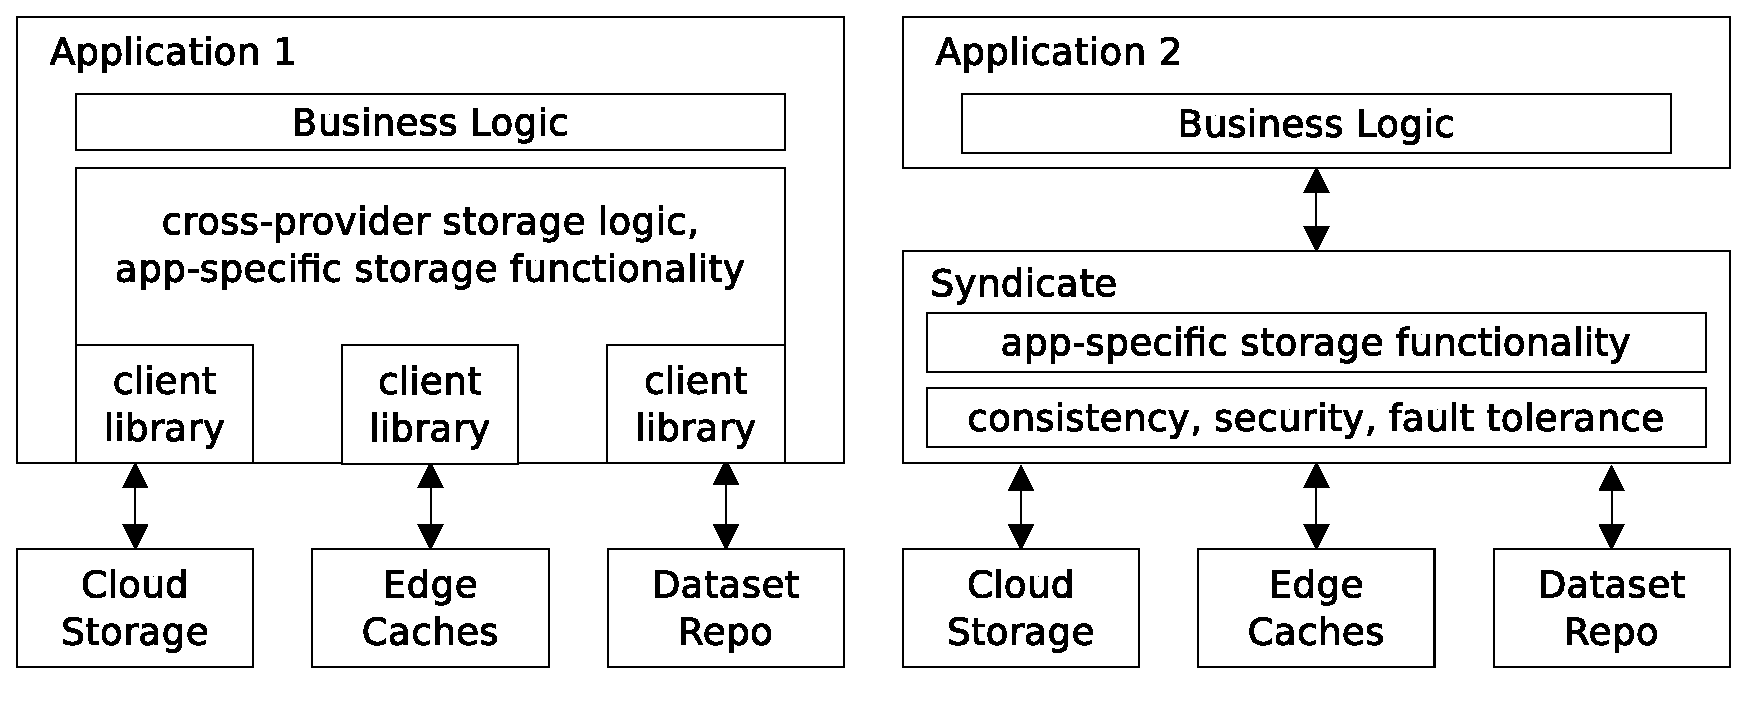
\includegraphics[width=0.47\textwidth]{figures/overview}
\caption{\it Application design with and without Syndicate.}
\label{fig:overview}
\end{figure}

Each type of component system offers well-understood
{\it functional} benefits.  Cloud storage offers an ``always-on''
repository for hosting a scalable amount of data, while keeping it
consistent and enforcing access controls.
Dataset repositories host and curate a scalable amount of read-only data on 
behalf of many applications.  CDNs, caching Web proxies, and HTTP object caches (``edge
caches'') help under-provisioned origin servers scale up the
volume of requests they can handle.
In all cases, instances of these systems ({\it providers}) make their 
functional benefits available through instance-specific APIs.

In contrast, the providers' infrastructure
offers two key \textit{utility} benefits transparently
---data durability and access locality.
Cloud storage and dataset providers improve durability by
replicating data to geographically distributed
datacenters, and edge caching providers improve locality by
placing temporary copies of data at sites closer to readers than the
origin servers (lowering latency and increasing bandwidth).

Unlike functional benefits, utility benefits can be aggregated.
Leveraging multiple providers yields more utility than leveraging any single
one, and improvements to one 
provider improve overall utility.
However, doing so is non-trivial because each provider
has a different API, with different functional semantics.  The developer
must design the application around this, thereby coupling its storage logic 
to provider implementations (Figure~\ref{fig:overview}, left).

Our key insight is that this coupling can be avoided by leveraging providers not for 
their functional benefits, but for the utility they offer---cloud
storage and dataset providers offer durability, and edge caching providers offer
locality.  While this strategy ultimately makes the developers responsible for storage functionality, doing so lets them
implement exactly the functionality they need while aggregating provider utility.
\Syndicate\ helps them implement and deploy this functionality at scale, while
minimizing provider coupling and addressing common storage concerns
on their behalf (Figure~\ref{fig:overview}, right).

The key contribution of \Syndicate\ is wide-area software-defined storage
service that runs on top of unmodified providers.  It provides an
extensible interface for implementing domain-specific storage
functionality in a provider-agnostic way, while addressing common cross-provider 
consistency, security, and fault-tolerance requirements automatically.
Using \Syndicate\ lets developers create a storage service for their applications 
that has the aggregate utility of multiple underlying providers, but without having to 
build and deploy a whole storage service from the ground up.
That is, \Syndicate\ creates virtual cloud storage through provider composition.

\section{Usage Scenarios}
\label{sec:motivation}

\Syndicate\ helps applications handle scalable
read/write wide-area workloads where cloud storage, edge
caches, and external datasets have complementary roles to play.  To motivate its
design, we explore three application domains that today are dominated by 
vertically-integrated storage point-solutions, and argue that the ideal 
storage system in each domain would be flexible enough to integrate 
a changing set of disparate providers into a coherent whole.  In doing so, 
it could allow applications to leverage providers 
for their utility benefits, independent of their functional benefits.
A concluding subsection summarizes our observations about these examples,
which influence our design.

\subsection{Scientific Datasets}

Tens of thousands of computers work together to process multi-terabyte
datasets; genomic sequencing datasets being illustrative
examples~\cite{GenBank,metagenomics,1000genomes}.
Researchers run small experiments in their labs on local workstations
and clusters, but run large experiments on powerful cloud computing platforms
and scalable grids of computers in the wide-area.
At the same time, they share findings with collaborators,
archive working datasets in cloud storage,
and submit vetted results for integration into the original datasets.

However, each provider has
different curation policies, APIs, performance profiles, consistency models, and 
access controls.  Grids and clusters must be specifically programmed 
to access each, or data must be manually staged for them.  This leads 
to point-solutions and manual procedures for sharing data.

Ideally, researchers would store relevant data on their
local workstations for fast access, and seamlessly stream it from
dataset providers on an as-needed basis (as in iRODS~\cite{irods}),
regardless of source.  The data would be accessible to a scalable
number of readers via edge caches (as in CERN VM-FS~\cite{cern-vmfs}),
provided that readers always receive fresh data.  Results from
authorized computers would be sanitized and uploaded to
researcher-chosen storage (as in Folding@Home~\cite{folding-at-home})
for subsequent curation.

\subsection{Collaborative Document Editing}

Collaborative document editing systems include cloud-hosted systems
like Google Docs~\cite{google-docs}, version control systems like {\tt
  git}~\cite{git}, and industry-specific form-processing systems such
as Blackboard~\cite{blackboard} and OpenEMR~\cite{openemr}.  In all
cases, the system lets a set of users read and write 
documents, subject to common format, consistency, and access control rules.

A key challenge is that users have different usage policies for their 
data.  For example, a doctor editing
medical records must keep a verifiable edit history and guarantee
confidentiality.  As another example, businesses sharing documents
through a third party must require edits to be mirrored to their own
servers for extra durability.

Ideally, users could bring their own storage system for hosting
writes.  The storage system would enforce the user's policies whenever
another user accesses it through the application.  At the same time,
the application would allow a scalable number of users to access
(fresh) data through edge caches, regardless of the underlying
storage.

\subsection{Virtual Desktop Infrastructure}

An alternative approach to giving employees corporate computers is to
let them bring their own devices, and have them run a corporate OS in
a VM while they are at work.  Employees download their VM images when
they begin the day, and periodically save their sessions until they
leave.  VDI systems exploit the facts that VM images do not change
much between sessions~\cite{collective} and have only one writer (the
user), in order to achieve scalable VM deployment through on-site VM
block caching.

While some VDI implementations (such as Citrix~\cite{citrix}) use system-specific
infrastructure, the ideal scenario is to let the corporation use the
cache and storage providers that best meet their business needs, and
impose their own user authentication requirements.  The VDI
infrastructure is not desirable if there already exists proven
in-house equivalents that can be used for the purpose.

\subsection{Observations}

Despite being point-solutions, the real-world examples above address reoccurring 
storage-level concerns.  These include stronger-than-eventual consistency, 
common fault tolerance strategies (such as automatic fail-over and integrity checks),
and common security requirements (such as access control and authentication).  This suggests 
that with the right refactoring, the mechanisms that address these 
concerns can be implemented once and reused across different application domains.

Our goal is for \Syndicate\ to provide a storage service that 
addresses these concerns for these and similar applications, while allowing developers
to dynamically extend it instead of rewrite it.  In doing so, developers could re-use \Syndicate\ as the 
storage layer to meet basic storage needs, and develop only the 
the extra storage functionality as a code module for \Syndicate\ to load and deploy.  This saves the effort of
creating multiple point-solutions, and creates an opportunity for re-using specialized 
storage functionality across \Syndicate-powered applications.  Once our goal is achieved, 
developers can use \Syndicate\ to combine providers to gain the utility benefits they offer, and not concern 
themselves with integrating their functional benefits into the application design.

There are three design challenges to achieving this goal.  First, \Syndicate\ must provide  
storage abstractions that allow the application to interact with data without 
coupling its design to underlying providers.  At the same time, the abstractions should 
couple \Syndicate\ to providers as loosely as possible.

Second, to facilitate reuse, \Syndicate\ must offer a storage programming model 
that distinguishes between logic that adds support for additional providers, and logic 
that adds provider-agnostic storage functionality (such as encryption or access logging)
or extends \Syndicate's built-in features.

Third, regardless of provider functional benefits and application extensions, \Syndicate\ must always meet consistency, fault-tolerance, 
and security requirements.  If needed, \Syndicate\ must make up for shortcomings in the design of underlying providers.
Once addressed, \Syndicate\ can aggregate their utility benefits.

%llp: talk about gateways, but not common/base functionality
%like consistency; although first paragraph of next section hits
%this, this paragraph somewhat minimizes Syndicate's role. Not
%sure how to address.

%Our strategy is to elevate these gateways to first-class logical
%storage components and make them programmable.
%The application would define its own storage functionality, and
%\Syndicate\ would distribute and run it in these gateways.  In doing
%so, we would reduce building storage point-solutions to writing only
%the logic that differentiates them from commodity providers.


\section{Design}
\label{sec:design}

As described in our motivation, there are two major aspects to StealthMail’s design.  The first is the subsystem for securely and automatically managing keys.  We refer to this subsystem as AutoKey.  The second is the protocol for sending and receiving emails, called Secure Message Request Protocol (SMRP).  SMRP relies on AutoKey to ensure the sender and receiver have the appropriate keys in place before communicating.

\subsection{Architecture}
Our design assumes Alice and Bob both have sets of trusted user endpoints that run loosely-synchronized clocks, and that each endpoint can access the user's personal cloud storage account for hosting hard state (across sessions).  Additionally, we assume that user endpoints can run code, in execution and resource contexts, outside of the web browser (such as in a VM).

Other than requiring users to have cloud storage, there are four main components of StealthMail (Figure~\ref{fig:overview}):\vspace{0.5em}

{\bf $\bullet$ Endpoint Daemon:} is a program that runs on the user endpoint, separately from the browser.  It performs key and session management, caching, cloud storage access, and cryptographic operations.\vspace{0.5em}

{\bf $\bullet$ Mail UI:} differs from a conventional webmail UI only in that it issues its RPCs to the locally-hosted \emph{endpoint daemon} instead of a remote webmail server. These two components are intentionally separated for practical reasons, because at the time of this writing there is no way to perform cryptography inside the browser without exposing the user to a multitude of Javascript-based attacks (code injection, XSS, and inter-tab leakage).\vspace{0.5em}

{\bf $\bullet$ StealthMail Server:} helps user endpoints discover new messages and assists with backwards compatibility.  It also serves copies of users' public keys, certificates, and storage signatures, which are mirrored by one or more metadata repositories.\vspace{0.5em}

{\bf $\bullet$ Metadata Repositories:} are not required for correct execution as they host redundant information, but using one or more of these increases the number of servers Mal must compromise.\vspace{0.5em}

The endpoint daemon, StealthMail server, and metadata repositories work together to implement the AutoKey system for key distribution. StealthMail servers along with cloud storage, and endpoint daemons work together to implement SMRP.  Figure~\ref{fig:overview} shows how this manifests in inter-component communications.

\begin{figure}[h!]
\centering
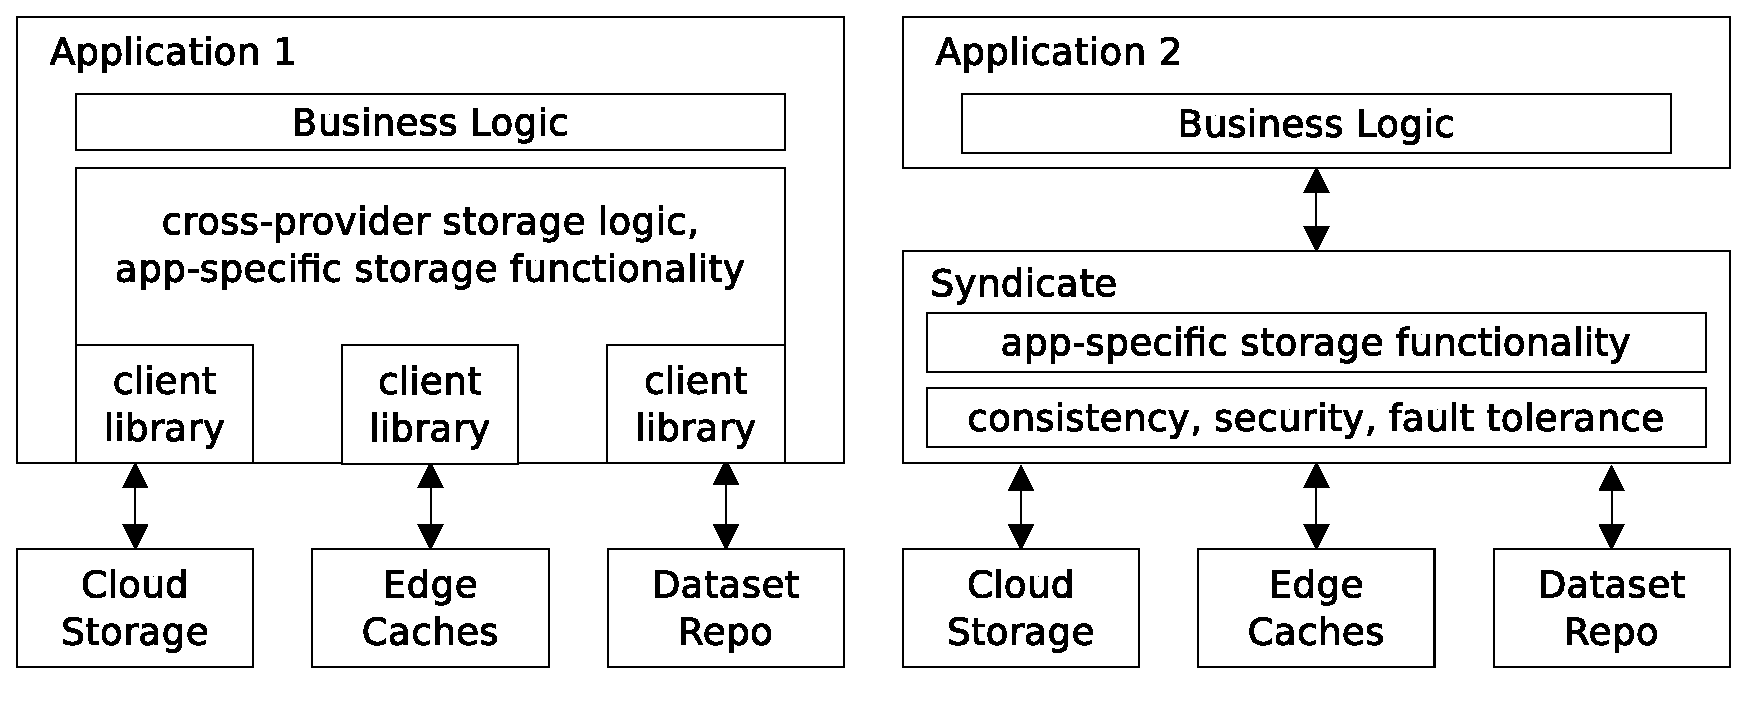
\includegraphics[width=0.5\textwidth]{figures/overview}
\caption{\it Overview of the StealthMail architecture, and various data flows that must take place before Alice sends a message to Bob.  Solid-head arrows are part of the AutoKey process.  Unfilled-head arrows are part of the SMRP process.}
\label{fig:overview}
\end{figure}


In AutoKey, each user is given an account public/private key pair, a storage public/private key pair, and one or more signing public/private key pairs.  The private keys are stored encrypted with the user’s password, and only decrypted when the device is running a session.  The account and signing public keys are made available in the form of certificates signed by the account private key.  The use for each key pair is listed in Table~\ref{tab:keypairs}.

\begin{table*}[ht!]
\begin{tabular}{ | l | p{14cm} |}
\hline
\textbf{Key Pair Name} & \textbf{Usage} \\
\hline
Account key pair & Certifying and revoking other public keys. \\
Storage key pair & Sealing/unsealing and signing cloud-hosted data.  Used for message confidentiality and state CIA. \\
Signing key pair & Signing email messages and attachments.  Used for message integrity and authenticity. \\
\hline
\end{tabular}
\caption{\it Names and usages for a user`s key pairs used in StealthMail`s AutoKey subsystem.}
\label{tab:keypairs}
\end{table*}


\subsubsection{Storage}
StealthMail protects the contents of cloud storage from tampering by replicating cryptographic signatures.  Each file uploaded to cloud storage is sealed with the user's storage private key for confidentiality.  StealthMail organizes the files into a Merkel tree, such that each directory contains the signed hash of all of its children's signed hashes.  Each hash is sealed by the storage private key, making external tampering from Mal evident.

Writing data is similar to two-phase commit.  A writer endpoint prepares to write by generating the new root signature, and replicating it to its StealthMail server and all metadata repositories.  If they all authenticate and accept it, the writer uploads the data to cloud storage, and then broadcasts a signed success message.  Write completes when the StealthMail server and metadata repositories acknowledge upon successful authentication.

Because reads and writes are serialized by the fact that the user does not use two endpoints simultaneously, the metadata repository only needs to store the last root signature it received.  To avoid timing out partway through writing, the endpoint splits large writes into smaller ones and commits them separately.

On read, the endpoint verifies the integrity of cloud storage by fetching the root signatures from these servers and comparing them to the one in cloud storage.  Because Mal cannot compromise all servers, and cannot compromise all channels, the reader will learn if Mal has tampered with a server if the signatures do not match.  These read and write protocols are executed by AutoKey to store trusted public keys in a tamper-evident way.

Given the threat Mal poses to the system, StealthMail employs a fail-fast approach to handling storage faults.  Unavailability or inconsistencies discovered in cloud-hosted data (such as incorrect signatures) are assumed to be due to external interference from Mal.  This is a reasonable trade-off, because it alerts users and cloud storage operators to Mal's presence.  In practice, StealthMail servers are deployed in highly-available infrastructure.

StealthMail is fundamentally a pull-based architecture and only the user's endpoints may write to the user's cloud storage,   Instead of sending data from Alice's endpoint to Bob's email server, Alice will write messages into her cloud storage, and Bob will download them later using SMRP.  This is a departure from SMTP, that can be used to build new features like an ``un-send mail'' feature and to economically disincentivize spam mail by requiring the sender to pay for storage.

\subsubsection{Usability}
A user interacts with StealthMail through the web browser, using the local endpoint as a web proxy.  The UI is stored as files in cloud storage and are signed by the storage private key.  This lets the endpoint verify their authenticity and integrity before serving them over the local trusted RPC channel, effectively preventing code injection attacks from Mal.

Before Alice or Bob can use StealthMail, they must set up the endpoint code.  However, we discuss strategies to facilitate this initial step in the section~\ref{sec:implementation}.  We assume in the following sections that the endpoints all run instances of the endpoint code in local VMs.

\subsection{Bootstrapping Trust}
Before Alice can use StealthMail, she needs an account.  In creating one, she bootstraps AutoKey by establishing her public key and registration date with each component, populating her cloud storage with initial application state, and granting her endpoint permission to access it.  She also establishes security questions and answers to be used to recover her private key, should she forget her password.

\begin{figure}[h!]
\centering
\includegraphics[width=0.5\textwidth]{figures/register}
\caption{\it The StealthMail key registration protocol.}
\label{fig:register}
\end{figure}

To do so, her endpoint replicates her account public key and backs up her revocation certificate to more servers than Mal can compromise.  We assume that Mal cannot alter the behavior of the servers during the registration process; if the servers do not behave correctly, the registration fails (Figure~\ref{fig:register}).

From a usability standpoint, creating an account on the StealthMail server is similar to doing so on a webmail server.  Alice begins by submitting a desired username and password to the StealthMail server through the endpoint, as well as any number of hard-to-guess security questions and answers, and the identifier for an uncompromisable out-of-band channel to confirm the registration (e.g. a phone number or existing email address).  The StealthMail-specific extra requirements are the authentication tokens needed to access her cloud storage, and her additional metadata repositories.

Once the information is entered, the endpoint uploads the username and password to the StealthMail server, which replies with a one-time-use registration URL via the out-of-band channel (we assume that Eve cannot determine the password in this step).  Alice navigates to the URL to complete her registration.  Once Alice confirms, the StealthMail server remembers iterated salted hash of the password and out-of-band channel identifier, so Eve and Mal cannot easily learn either and so Alice can use the channel identifier later to reset her password.

Once Alice’s account is created on the StealthMail server, the endpoint sets up her keys and certificates.  It generates her public/private key pairs, and signs the storage and signing public keys with the account private key.  It then generates revocation certificates for the account and storage keys, as well as two public certificates---one for the signing key, and one for the storage key---that contain Alice’s username, the public key, the timestamp, and a nonce for uniqueness (``pubkey certs'' in Figure~\ref{fig:register}).  It signs these certificate with the account private key.

It then proceeds to replicate the account public key and certificates to each server, using the StealthMail server to vouch for her.  To upload them to the StealthMail server, It generates an HMAC over them using the password as the shared secret.  Once the StealthMail server validates and accepts them (remembering the nonce to prevent re-register attacks), the endpoint uploads them to each metadata repository.  The endpoint authenticates to each using OpenID protocol and Alice’s password, where the StealthMail server acts as the OpenID provider.  The metadata repositories do not consider a revocation certificate to be in force until Alice activates it later.

The endpoint finishes by populating Alice’s cloud storage with StealthMail account state, using the authentication tokens she supplied at the beginning of the process.  It uploads her public key certificates as a world-readable files in cloud storage (for Bob to download later) as well as her revocation certificates and account public key (which are NOT encrypted).  It encrypts the private keys and cloud storage credentials using an authenticated symmetric key scheme, deriving symmetric keys from her salted password.  It also seals a copy of the storage private key with the answers to her security questions, so Alice can change her password without losing her data.  The endpoint uploads the security questions and sealed keys to cloud storage, seals the MACs and salts from the encryption with the password, and erases them from RAM, completing the registration and AutoKey bootstrap process.

\subsection{Session Management}
Once AutoKey is bootstrapped, Alice can use multiple endpoints to access her account transparently.  To do so, Alice simply enters her username/password, and the endpoint (via AutoKey) fetches her sealed storage private key, endpoint-specific sealed signing private key, and sealed cloud storage credentials.  For a new device, the endpoint generates a new signing key certificate and revocation certificate for it, seals the private key with the password, and distributes the certificates to the StealthMail server and metadata repositories (which authenticate them with the account public key they obtained on registration).  The servers do not publish the revocation certificates until Alice signals them to do so.

Alice can specify that a user endpoint will be used for only one session (akin to a ``This device is public'' checkbox in webmail).  If so, the signing key will have an expiration date in the very near future, e.g. 30 minutes.

When Alice logs out or her session times out, the endpoint has AutoKey erase any secrets from RAM.  As a precaution, it also erases any data it cached data, and will erase cached data automatically if it restarts. Cached data is always sealed with one of Alice's public keys before being written to local storage, preventing Eve from breaking confidentiality via offline analysis.

\subsection{Key Distribution}
In AutoKey, Bob's endpoint must learn Alice's account, storage, and signing public keys before he can communicate with her.  Once it has them, AutoKey puts them into his cloud storage, executing the two-phase write protocol so his other endpoints can securely and automatically fetch them later.  The challenges are in obtaining them for the first time in such a way that Eve and Mal cannot trick him into learning the wrong ones, and in revoking trust in them without also being tricked.

Bob's endpoint will trust one of Alice's public keys only if AutoKey can get unanimous agreement on the key's value from each server that hosts them, and only if the key is not expired.  Similarly, AutoKey will check for an activated revocation certificate if all servers agree on the same key, and the key is different from the currently trusted key.  This strategy works under our threat model because without Alice's password, Mal is not powerful enough to send the wrong key on every channel, or change it to every server.

While Bob trusts the keys, AutoKey periodically checks to see if it Alice's servers have changed them.  Because the account public key and storage public key do not change as often as the signing key (see the next section), it will check the account key at most once per session.  However, it will check the storage and signing public keys every time Bob sends a message to Alice.

To advertise her keys, Alice's StealthMail address is a well-formed email address that indicates her username, her cloud storage provider, her StealthMail server, and any metadata repositories that host her keys.  We use the character ‘\^’ to separate them---for example, Alice's StealthMail address might be alice\^cloudstorage.com\^keybackup.org@mail.net, indicating that her data is hosted at cloudstorage.com, her keys are replicated to keybackup.org, and her StealthMail server is mail.net.  Each service makes both the keys and certificates available via canonical URLs derived from the username and the service name.  Bob's endpoint has AutoKey use TLS-secured channels with authenticated cipher suites (i.e. AES-GCM) to fetch copies from each service, in order to hedge against external tampering from Mal (but not eavesdropping from Eve).

In the event that some of Alice's services are unreachable, AutoKey continues to trust Bob's copies of Alice's public keys even if there is disagreement among the online servers.  This is to prevent Mal from weakening the system with denial-of-service attacks.  In practice, Alice's services run on highly-available infrastructure, so unreachability problems will be rare and transient.

\subsection{Key Revocation}


\begin{figure}[h!]
\centering
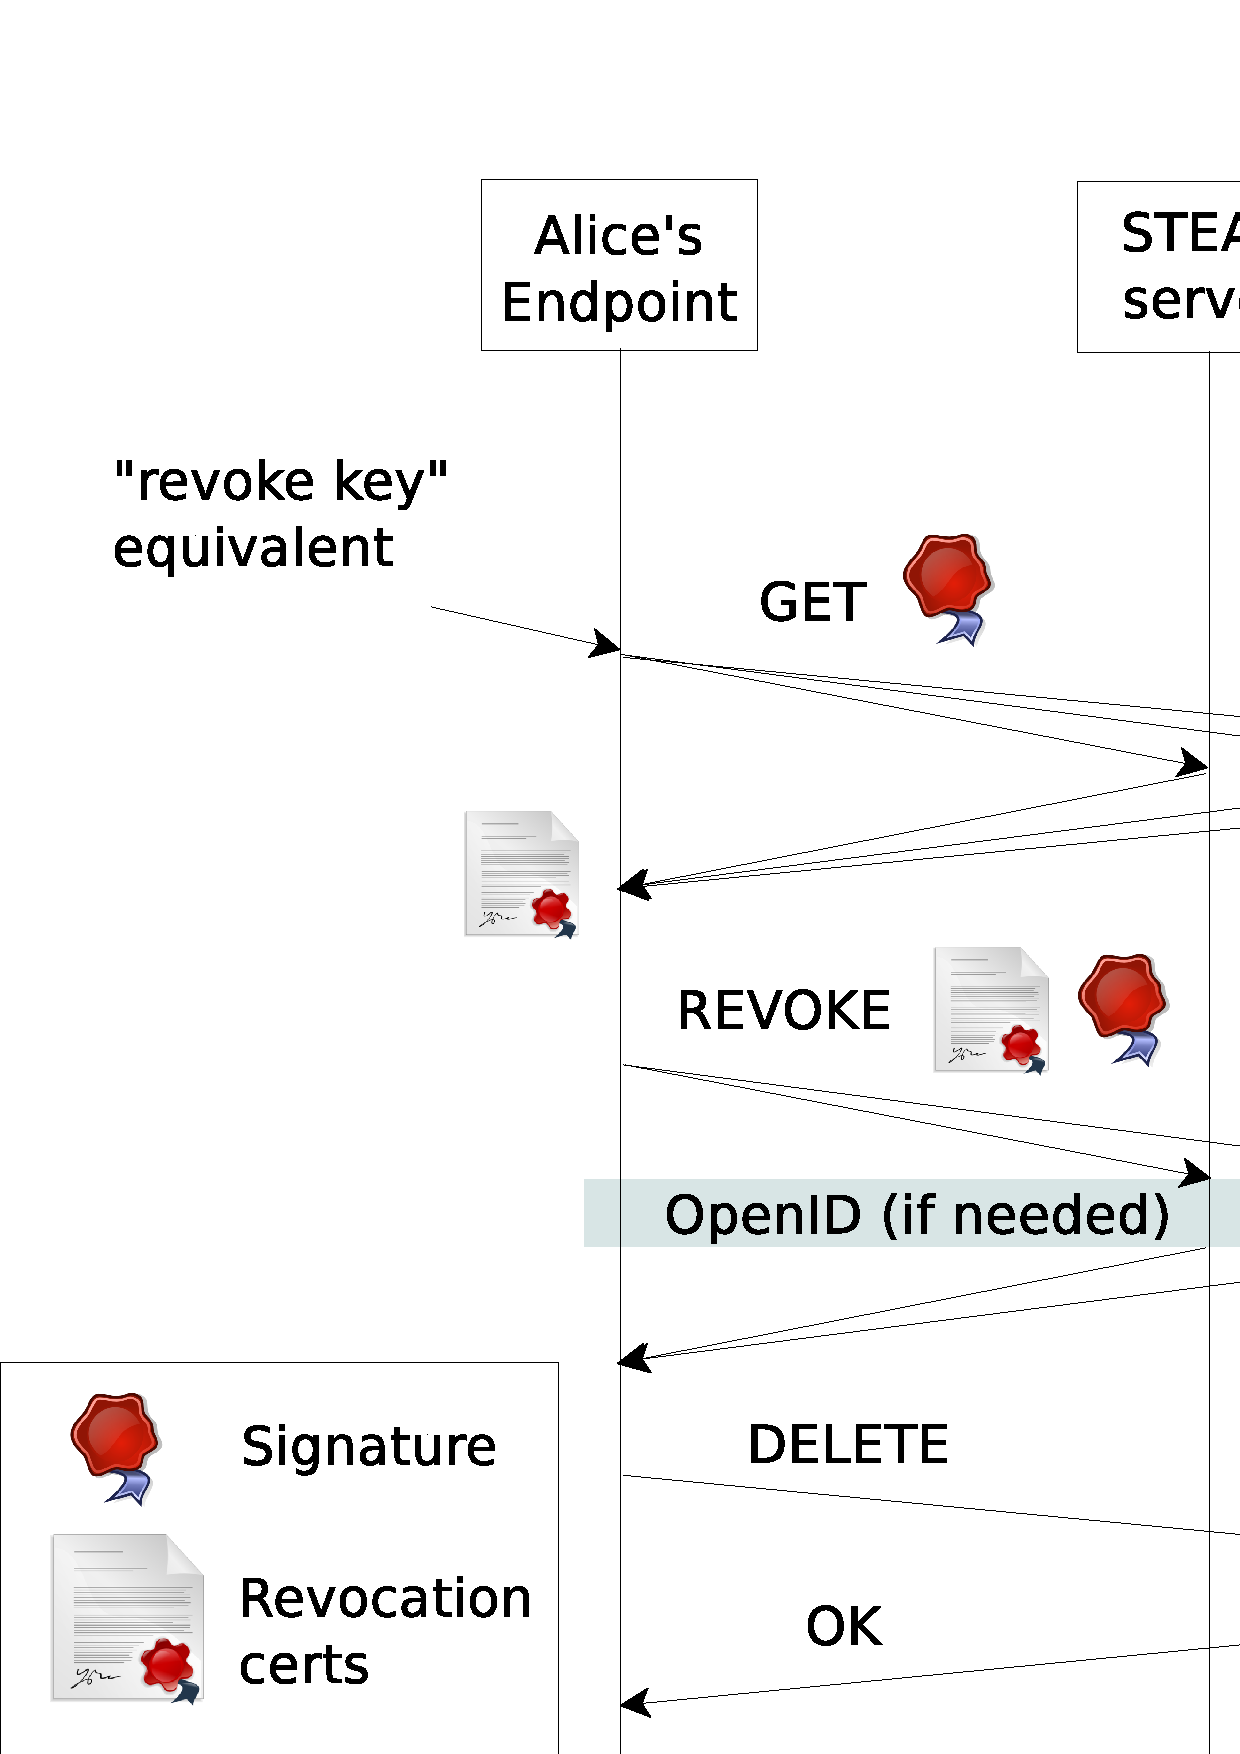
\includegraphics[width=0.5\textwidth]{figures/revoke}
\caption{\it The StealthMail key revocation protocol.}
\label{fig:revoke}
\end{figure}

Inevitably, AutoKey will need to revoke Alice’s keys for her.  When Alice removes access permission from a trusted endpoint device, AutoKey revokes its signing key.  When she changes or resets her password, AutoKey revokes and regenerates her keys by default because the reason for doing so may be due to a password compromise.

Revoking a signing key is a matter of activating its stored revocation certificate (Figure~\ref{fig:revoke}).  To do so, AutoKey first obtains it by downloading it from each the servers, using a request signed by the account private key.  It also gets a copy from cloud storage.  At least one of the servers will reply with the correct revocation certificate, since Mal cannot compromise all of them under our threat model.

AutoKey then re-uploads it in a signed request to the servers, indicating that the should publish it.  The servers erase the old public key certificate on successful verification, and AutoKey removes it from cloud storage.  Then, when Bob contacts Alice next, his endpoint will detect the key discrepancy, discover the revocation certificate, and stop trusting the old signing key.

If Eve compromises Alice’s password, she will be able to read her incoming messages, and messages sent to others.  If Mal compromises Alice’s password, she can do anything with the account.  To regain control, Alice resets her password, effectively re-registering her account and re-bootstrapping AutoKey using registration protocol described earlier (but with two small differences described below).  As before, we assume that Mal cannot alter the behavior of the servers during re-registration.

Unlike with first-time registration, the StealthMail server requires Alice to submit the same out-of-band communication channel as she did before.  Also, AutoKey sets a flag while uploading new public key information to ask for a reply containing the old revocation certificate.  It also obtains the copy uploaded earlier from cloud storage, and then executes a variant of the signing key revocation protocol to publish the revocation certificates for her account and storage keys.  The only differences are that the revocation certificates will be signed by the new account key, and that the servers will additionally verify the request with OpenID to ensure that it came from Alice (the only person who knows the new password).

When Alice logs in next, her endpoint ``imports'' her old account data by unsealing it with the old storage key and re-sealing it with the new storage key.  If Alice remembers her old password, her endpoint decrypts the old storage key automatically.  If she does not, her endpoint obtains the copy of the storage key sealed with the answers to her security questions, and prompts her for them to decrypt it.

Deleting an account is similar to revoking the keys.  The only difference in the process is that no new keys are generated.

\subsection{Sending, Receiving, and Un-Sending}
Once Alice and Bob have exchanged public keys with AutoKey, they communicate with SMRP, described in this section.  In SMRP, Alice sends Bob a message by sealing it with his storage public key, uploading it to her cloud storage, and making it world-readable. Bob’s endpoint downloads and decrypts it, sanitizes it, and serves it to Bob’s browser for him to read. The same principle applies to attachments, which in StealthMail are sent as separate files to be downloaded.  Alice makes a copy for herself in her ``sent'' folder, if desired.

If Bob expects email from Alice, he can search Alice’s cloud storage for new messages and fetch them.  The UI allows him to query individual contacts for new messages.

The challenge for Bob is to discover when Alice sent him an unsolicited message.  To address this in SMRP, Bob’s StealthMail server acts as a notification service for new email.  Alice sends Bob's StealthMail server a message metadata record, sealed with his storage public key and signed with her signing private key, that identifies herself as the sender and Bob as the recipient.  It serves as a hint to Bob that he has unsolicited mail, and tells him the message recipients, the subject, the human-readable names of the attachments, and the attachment signatures.  This information is hidden from the StealthMail server to provide end-to-end message CIA, and its small size makes it easy for it to store many of them.

When Bob accesses his email, his endpoint downloads and decrypts the unread message metadata records from the server.  Each of them appear in Bob's UI as unread messages. The UI tells Bob the subject, recipients, and attachment names.  Once Bob's endpoint reads and stores the metadata records, the StealthMail server is free to erase them.  

When Bob opens an unread message from Alice, his endpoint downloads, decrypts, and verifies the authenticity and integrity of Alice's message body, using the public keys obtained by AutoKey. Once verified, Bob reads it via the UI. To download an attachment, the endpoint streams it from Alice's cloud storage, verifies it, decrypts it, and delivers it to the UI as a file download.  As a performance optimization (and to assist automatic spam filtering), the endpoint prefetches message bodies as they are discovered.

Mailing lists in SMRP are treated like user accounts.  The only difference is that every participant on the list has a sealed copy of the account storage key and a personal signing key.

In SMRP, Alice can ``un-send'' a message by erasing the body and attachments from cloud storage.  This allows her to withdraw messages sent in haste, or sent accidentally to unintended people.  Bob will discover that she deleted it (i.e. he will receive a metadata record for a message that does not exist), but this may be preferable to having Bob read the entire message.  As such, once Bob obtains a message’s body and attachments, his endpoint replicates them to his cloud storage by default to keep them available even if Alice deletes it later.

\subsection{Searching, Tagging, and Filtering}
Beyond sending and receiving email, webmail users expect automatic spam filtering, the ability to organize messages and conversations, and the ability to search them.  In traditional webmail systems, this functionality resides on the server.  The challenge in providing it in StealthMail is in moving it to the endpoint to preserve confidentiality, but without compromising features.

Tagging messages is a matter of associating a given message with a bag of tags that Bob defines.  Bob’s endpoint incrementally builds an index that pairs each tag to a list of message identifiers.  To search messages by tag, the endpoint fetches a page of the tag’s index, looks up the messages, and serves them to the UI.

To search messages, the endpoint incrementally builds a search index as Bob reads them, using an off-the-shelf indexer.  The indices are updated and synchronized with cloud storage in the background as he opens and reads messages.  As a performance optimization, the endpoint lazily downloads the index by chunk they are needed by the indexer.  It caches them for the session, and asynchronously replicates modifications.

To filter messages, the endpoint uses a combination of a locally-trained classifier and sender blacklists.  Bob has the option of marking messages as spam and marking senders as spammers, in which case the endpoint feeds the message body into its local spam classifier and replicates the classifier’s new model parameters to cloud storage.  This allows the classifier to be used across endpoints without revealing its parameters.  If Bob marks a contact as a spammer, AutoKey revokes trust in its public key, and the endpoint will ignore future messages from it.

Using only a local spam filter is desirable for confidentiality.  The spam classifier model parameters can leak information about the contents of the messages they have classified, so it is important that Bob’s endpoint not share this information directly.  This is in contrast to webmail providers today, which learn to classify spam by monitoring many user accounts.  However, empirical tests~\cite{local-spam-filter-eval} suggest that existing local spam filters can achieve upwards of 98\% effectiveness in practice, suggesting that our strategy should not significantly impact usability if the endpoint code ships with a pre-trained classifier.

\subsection{Backwards Compatibility}
Because email is already a widely-used service, StealthMail must remain backwards compatible with it to allow Alice and Bob to communicate with Charles, a user who relies on conventional email.  To do so, the StealthMail server provides an SMTP/SMRP gateway that translates one protocol into the other.  The StealthMail server has its own cloud storage to hold messages from Charles to serve to Alice via SMRP.  Alice’s messages to Charles are automatically routed through SMTP because Charles does not have a well-formed StealthMail email address.

The gateway alone does not provide \emph{CIA guarantees}.  If Charles wants a limited degree of CIA, StealthMail offers one of two options that require a minimal change in his workflow.  First, if Charles uses PGP already, he will send his public key and encrypted messages via SMTP.  AutoKey obtains Charles’ public key automatically.  While this is less trustworthy than StealthMail’s approach, it is better than nothing, because Mal has only one very short window of time to alter the public key.

If Charles does not use PGP, he must first agree with Alice on a shared secret out-of-band, and assume that Mal does not compromise the StealthMail server or the TLS CA server that vouches for its TLS public key.  To send her a message securely, he navigates to her StealthMail server, enters the secret, and is given a webmail form for composing her a message.  When he submits his message, StealthMail it available to Alice via SMRP.

When Alice replies via SMRP, the StealthMail server sends Charles a URL instead of the message body.  When opened, the StealthMail server gives him a specially-crafted HTML page that contains Alice’s ciphertext, a decryption algorithm in Javascript, and a secret submission form.  When Charles enters the secret, the page decrypts the message for him.

\section{Implementation}
\label{sec:implementation}

Building \Syndicate\ resulted in two important artifacts: a generic
and scalable Metadata Service, and a ``narrow waist'' interface
between applications and providers.

The first, which includes a client-side library, let an
application use unchanging URIs (i.e. object paths) to download guaranteed-fresh mutable
data from underlying caches, without relying on them for consistency.
The client library manages manifests and caching, and provides 
an API for uploading new metadata.

To scale on top of a NoSQL store while providing filesystem-like metadata 
consistency, the \MS\ divides a record into
into a seldom-written ``base'' record, and a set of often-written ``shard'' records.
Writes are distributed across shards, so the \MS\ can batch outstanding writes
regardless of how long an individual {\tt put} operation in the store takes.
They are recombined into a whole record by selecting the shard with the largest 
last-write timestamp, providing last-write-wins write semantics.  Base records are 
transactionally created to prevent name conflicts.

% Definitely want a figure of this next paragraph.
% If the reader remembers anything from this paper,
% it should be this and the consistency protocol.
% -jcn
The second artifact is an application-controlled cloud
abstraction layer, which forms a ``narrow waist''
between applications and providers.  This facilitates rapid storage service 
deployment by reducing the task of creating a custom storage system to deploying
the appropriate \SGs.  It also facilitates 
independent provider evolution by reducing the task of supporting legacy applications
to providing the $R$ and $W$ that lets them continue to
leverage the provider in the face of otherwise-incompatible changes.

% Do these next two paragraphs belong in the Design section?
% -jcn
Broadly, there two deployment models for \Syndicate, depending on whether 
or not the application is peer-to-peer or client/server.  In the first model, 
each peer runs a write- and coordinate-capable \SG.  This is the deployment 
model we use today on PlanetLab~\cite{PlanetLab}.

In the second model, application servers run write- and coordinate-capable \SGs,
and a scalable number of clients run read-only \SGs\ and send writes directly to 
application servers.  This model dovetails with Web
application design, where Web page (client) does not write to the storage tier 
(server \SG) directly, but instead sends data to the application tier to write 
it on its behalf.

In both cases, Replica \SGs\ may be colocated with User \SGs, or deployed
in a separate cluster.  The former horizontally scales 
writes to cloud storage, but consumes extra application resources.  The latter provides the 
cost and security benefits of a dedicated, isolated storage tier,
but at the expense of one more network hop per write.

\section{Evaluation}

Our usability goal has been to preserve the semantics of webmail while offerring transparent end-to-end CIA.  To evaluate this, we consider the steps and information required to complete common webmail tasks, and compare them to how STEAK and PGP perform them.  These include setting up and destroying an account, adding and removing a contact, sending and receiving messages, and changing account passwords.

In evaluating against PGP for usability, we use the user’s guide for PGP 7.0 as a baseline comparison.  We also consider approaches taken by Enigmail, Mailpile, and Mailvelope, which seek to make PGP easier to use for securing email.  We show that while STEAK does not offer exact webmail semantics, it offers semantics much closer to webmail than even user-friendly PGP implementations.

At the same time, our performance goal for STEAK is to avoid hindering responsiveness to user interaction.  Our preliminary evaluation shows that running AutoKey asynchronously hides the time needed to perform key distribution, and that encryption and decryption do not significantly increase latency.

\subsection{Endpoint Management}
Assuming the web browser is already installed, setting up webmail takes no effort from the user.  However, because performing encryption in server-chosen Javascript with no validation is unsafe, both PGP and STEAK require an additional software component to be installed on each endpoint.  While this can be simplified with the endpoint device's app store, a PGP user must also create a subkey for each device, and sign it with the master key.

\begin{table}[ht!]
\begin{tabular}{ | L{2.0cm} | L{4.5cm} |}
\hline
\textbf{Webmail} & \textbf{STEAK and PGP} \\
\hline
(None) &

\vspace{-3mm} 
\begin{enumerate}
  \item{Install endpoint software.}
  \item{(PGP) generate and sign subkey.}
\end{enumerate} \\

\hline
\end{tabular}
\caption{\it Steps to set up an endpoint.}
\label{tab:account-creation}
\end{table}

Destroying an account in webmail and STEAK are equivalent--the user navigates to the page in the UI to do so, and enters the username and password.  The rest is automated.  In PGP, the email account must be destroyed separately from the key.  The private keys must also be erased, and the public keys revoked.

\subsection{Account Management}
Registering an account in STEAK has a similar workflow to registering a webmail account; the only difference is that STEAK users must also submit cloud storage authentication tokens and additional metadata repositories (if desired).

By contrast, a PGP client requires the user to create an email account before configuring it, making the task at least as difficult as webmail.  It additionally requires users to generate keys and revocation certificates, and export the public key (e.g. to a key server).  While it is possible to integrate this into the account registration process (the approach taken by Mailpile), the user is inevitably involved in the key setup process because she will need to learn how to sign and trust other users’ keys. 

\begin{table}[ht!]
\begin{tabular}{ | L{3.5cm} | L{3.5cm} |}
\hline
\textbf{Webmail and STEAK} & \textbf{PGP} \\
\hline
\vspace{-3mm}
\begin{enumerate}
  \item{Navigate to provider URL.}
  \item{Submit username, password, out-of-band channel (STEAK: also cloud storage creds and metadata repositories).} 
  \item{Activate account with information sent on out-of-band channel.}
\end{enumerate} 
\vspace{-\topsep}&

\vspace{-3mm}
\begin{enumerate}
  \item{Create email account (steps 1-3 in webmail).}
  \item{Configure PGP client to use the email account.}
  \item{Generate and encrypt keys.}
  \item{Generate revocation cert.}
  \item{Publish pubkey.}
\end{enumerate} 
\vspace{-\topsep}\\

\hline
\end{tabular}
\caption{\it Steps to create an account}
\label{tab:account-creation}
\end{table}


Changing or resetting a password in STEAK is a matter of either submitting the old password or answering the security questions, and waiting for the account state to be re-sealed.  This is similar to webmail’s semantics.  While some PGP implementations offer a key recovery option using security questions, it must be manually enabled.  Moreover, the user must manually change the key password after recovering the key.


\begin{table}[ht!]
\begin{tabular}{ | L{3.5cm} | L{3.5cm} |}
\hline
\textbf{Webmail and STEAK} & \textbf{PGP} \\
\hline
\vspace{-3mm}
\begin{enumerate}
  \item{Go to to reset form.}
  \item{Answer security questions.} 
  \item{Obtain reset URL out-of-band.}
  \item{Enter new password.}
  \item{(STEAK) Wait for re-sealing.}
\end{enumerate} 
\vspace{-\topsep} &

\vspace{-3mm}
\begin{enumerate}
  \item{Enable key recovery option.}
  \item{Contact recovery server.}
  \item{Answer security questions.}
  \item{Change key password.}
\end{enumerate} 
\vspace{-\topsep} \\

\hline
\end{tabular}
\caption{\it Steps to reset a password.}
\label{tab:account-creation}
\end{table}

Deleting an account in webmail is as simple as entering one’s password and confirming the request.  This is also the case in STEAK, where all public keys are automatically revoked once the request is confirmed.  In PGP, however, the user must not only delete the email account, but also any private keys associated with it.  The user must erase the public keys from the key servers, and publish revocation certificates for the private keys.

\subsection{Contact Management}

Adding a contact in webmail is usually a matter of filling out a form, if it is not done automatically.  At a minimum it requires an email address and a name, but other fields are possible.

With PGP, the user must obtain, verify and trust a public key as well.  Mailpile attempts to reduce this to scanning QR codes or obtaining them from email headers, but nevertheless the user must make a choice on the trustworthiness of the peers who signed it.  Applying TOFU semantics makes it easier to use but less secure than STEAK, because there is only a single source for the key.  Moroever, PGP users must periodically re-acquire keys when old ones expire.

AutoKey lets STEAK obtain keys automatically and keep them fresh.

\begin{table}[ht!]
\begin{tabular}{ | L{3.5cm} | L{3.5cm} |}
\hline
\textbf{Webmail and STEAK} & \textbf{PGP} \\
\hline
\vspace{-3mm}
\begin{enumerate}
  \item{Open new contact.}
  \item{Add name, email.} 
  \item{Save.}
\end{enumerate} 
\vspace{-\topsep} &

\vspace{-3mm}
\begin{enumerate}
  \item{Open new contact.}
  \item{Add name, email.}
  \item{Obtain, verify, and trust pubkey.}
  \item{Save.}
  \item{Repeat 3-5.}
\end{enumerate} 
\vspace{-\topsep} \\

\hline
\end{tabular}
\caption{\it Steps to add a contact.}
\label{tab:account-creation}
\end{table}

\subsection{Accessing, Sending, and Receiving Email}

Accessing email from multiple devices is trivial in webmail if the device has a web browser.  It is equivalently easy in STEAK and PGP once the endpoint code is installed and set up.

Sending a message in webmail is a matter of opening a window to compose it, selecting the recipients, and sending it.  However, PGP implementations require the user to at least click through UI elements to encrypt and sign the message.  This is because only the user knows whether or not the recipient will be capable of decrypting the ciphertext.  STEAK's transparent backwards compatibility lets users avoid this, akin to webmail.

\begin{table}[ht!]
\begin{tabular}{ | L{3.5cm} | L{3.5cm} |}
\hline
\textbf{Webmail and STEAK} & \textbf{PGP} \\
\hline
\vspace{-3mm}
\begin{enumerate}
  \item{Open compose window.}
  \item{Select recipients.} 
  \item{Type body, add attachments.}
  \item{Send message.}
\end{enumerate} 
\vspace{-\topsep} &

\vspace{-3mm}
\begin{enumerate}
  \item{Open compose window.}
  \item{Select recipients.}
  \item{Type body, add attachments.}
  \item{Encrypt and sign.}
  \item{Send message.}
\end{enumerate} 
\vspace{-\topsep} \\

\hline
\end{tabular}
\caption{\it Sending a message.}
\label{tab:account-creation}
\end{table}


Reading a message in webmail is a matter of selecting the unread message.  This is also the case in STEAK-to-STEAK communication, and STEAK/SMTP communication where no CIA is needed.  Even in STEAK/SMTP communication with limited CIA, submitting a shared password to access a message is not a foreign concept.

PGP implementations can decrypt messages automatically if the key is known.  However, the user may be prompted to obtain and trust the key if not.

\begin{table}[ht!]
\begin{tabular}{ | L{3.5cm} | L{3.5cm} |}
\hline
\textbf{Webmail and STEAK} & \textbf{PGP} \\
\hline
\vspace{-3mm}
\begin{enumerate}
  \item{Select message.}
  \item{(STEAK/SMTP): submit CIA secret.}
\end{enumerate}
\vspace{-3mm}
 &

\vspace{-3mm}
\begin{enumerate}
  \item{Select message.}
  \item{If not trusted, obtain, verify, and trust pubkey.}
\end{enumerate} 
\vspace{-\topsep} \\

\hline
\end{tabular}
\caption{\it Reading a message.}
\label{tab:account-creation}
\end{table}

\subsection{Performance}

Keeping latency as low as possible is important for the user experience.  Our strategy for doing so is to perform as much work asynchronously as possible, so as to not keep the user waiting.  However, encrypting messages must occur synchronously, because the user expects messages to be sent as soon as the "send" command is given.


\section{Related Work}
\label{sec:related-work}

STEAK falls into the growing body of work relating to HCI in information security.  Barriers
to using secure email include lack of technical aptitude~\cite{why-jonny-cant-encrypt}
~\cite{garfinkel-email-survey}, and
stigmatization of chronic use~\cite{crypto-adoption-criteria}.

There have been several attempts to create usably secure email.
The simplest approach is incorporating key management functions into the 
UIs of existing email clients, as done by Enigmail~\cite{enigmail}.
More sophisticated variants of this approach perform automatic decryption
and verification, and recent variants like Mailpile~\cite{mailpile} attempt
to streamline key distribution and key fingerprint verification.  However, they do not
succeed in making the process transparent---the user is still involved in
trusting, verifying, generating, distributing, and revoking keys.

A more sophisticated approach is to automate key generation and distribution,
as seen in systems like ESCAPE~\cite{escape} and ePOST~\cite{epost}.
In these systems, a user's host generates a key and one or more trusted CAs
automatically vouch for it, allowing users to bootstrap trust in one another.
However, this approach assumes the CAs are never compromised, and requires them
to decide when to revoke keys.
In contrast, STEAK trusts CAs only for registration and backwards
compatibility, and revokes keys when users believe 
their passwords are compromised.

Another approach is ID-based cryptography, whereby system components
derive a user's public key from her identity~\cite{id-based-cryptography}.  This 
eliminates the need for PKI and public key distribution.  However,
revoking unexpired keys is infeasible---either the user must change 
her identity, or the master private key (and all other public keys) must be 
regenerated.

We consider STEAK's architecture to be an incremental improvement on
the Internet Mail 2000~\cite{im2k} proposal.  We take advantage of cloud storage 
independent of the user's ISP, while also addressing security and ubiquitous
access in addition to disincentivizing spam.

\section{Conclusion}
\label{sec:conclusion}

We have presented STEAK, a backwards-compatible email system that gives users 
webmail-like access semantics while providing message CIA guarantees.  It does so
by leveraging a user's cloud storage for hosting state, and by distributing and revoking
keys using more servers and channels than adversaries can compromise.  Our prototype
is under active development, but is qualitatively easier to use than PGP and does 
not hinder user-perceived performance.


%\comment{
\section{Acknowledgements}

We wish to thank Sapan Bhatia and Andy Bavier for their assistance on technical matters
such as preparing VICCI slices to run Hypercache and FUSE filesystems, as well as providing
guidance on building back-end on Hypercache to interface with public slice-federation architectures
such as VICCI.  We also wish to thank G\"{u}rer \"{O}zen, \c{C}a\u{g}lar Onur, Baris Metin, and Marc Fiuczynski
for their technical assistance in configuring and deploying Hypercache on VICCI.  Additionally, we
wish to thank Verivue, Inc. for allowing us to run their CDN implementation on a publicly-accessible
testbed.
}



{\footnotesize \bibliographystyle{acm}
{\bibliography{bibdata.bib}}


\end{document}







